% Exemple de fichier fonctionnnant avec la classe CAp2012.cls
% Base :
%	Classe pf2010.cls adpatée de pf2003 par Jean CHarlet
%	Classe pf2003.cls adpatée de ic2001 par Jean CHarlet
%
% 	Classe ic2001.cls adpatée de EEGDRI3 par Jean CHarlet
%
% 	Classe EEGDRI3.cls adpatée de ic2000 par Jean CHarlet
%
% 	Classe IC'2000 (ic2000.cls) par Jean Charlet
%
% 	adaptée de la classe IC'99 (afia99.cls) développée par Fabien Torre

%\documentclass{CAp2012}
\documentclass[publibook-draft]{CAp2012}

\newcommand{\verbfichex}{CAp2012.\xspace}
\newcommand{\verbfichclass}{CAp2012.cls\xspace}
\newcommand{\verbfichbst}{CAp2012.bst\xspace}


%\usepackage[pdftex]{pstricks}

\usepackage{verbatim}
\usepackage{subfigure}
\usepackage[french]{babel}
\usepackage[utf8]{inputenc}
\usepackage[T1]{fontenc}
\usepackage{mathtools}
\mathtoolsset{showonlyrefs=true}
\usepackage{amssymb}
\usepackage{natbib}
\usepackage{caption}
%%% francisation des algorithmes


%\newtheorem{algorithm}{Algorithme}
\newtheorem{definition}{Définition}
\newtheorem{lemme}{Lemme}
\newtheorem{theorem}{Théorème}
\newtheorem{hypo}{Hypothèse}
\newtheorem{cor}{Corollaire}
\newtheorem{prop}{Proposition}
\newtheorem{exemple}{Exemple}
\newtheorem{remarques}{Remarques}
\newtheorem{remarque}{Remarque}
\newtheorem{problem}{Problème}
\newtheorem{algo}{Algorithme}
\newtheorem{preuve}{Démonstration}
\newcommand{\argmax}{\operatorname*{argmax}} %\operatorname* pour les op. pouvant admettre des limites...
\newcommand{\argmin}{\operatorname*{argmin}}
\newcommand{\minp}{\operatorname*{min_+}}
\newcommand{\dom}{\operatorname*{dom}}
\newcommand{\Ker}{\operatorname*{Ker}}
\newcommand{\trace}{\operatorname*{trace}}
\newcommand{\cov}{\operatorname{cov}}
\newcommand{\epi}{\operatorname{epi}}
\newcommand{\card}{\operatorname*{Card}}
\newcommand{\conv}{\operatorname*{Conv}}
\newcommand{\vect}{\operatorname*{Vect}}
\newcommand{\var}{\operatorname{Var}}
\newcommand{\diag}{\operatorname{diag}}
\newcommand{\erf}{\operatorname{erf}}
\newcommand{\bound}{\operatorname*{bound}}
\newcommand{\vpi}{\operatorname{VPI}}
\newcommand{\gn}{\operatorname{Gain}}
\newcommand{\p}{\operatorname{Pr}}
\newcommand{\mlp}{\operatorname{MLP}}
\newcommand*\tto[2]{\smash{\mathop{\longrightarrow}\limits_{#1}^{#2}}}
\newcommand*\ntto[2]{\smash{\mathop{\nrightarrow}\limits_{#1}^{#2}}}
\newcommand{\X}{\mathbf{X}}
\newcommand{\Q}{\mathbf{Q}}
\newcommand{\A}{\mathbf{A}}
\newcommand{\Z}{\mathbf{Z}}
\newcommand{\Y}{\mathbf{Y}}
\newcommand{\E}{\mathbf{E}}
\newcommand{\K}{\mathbf{K}}
\newcommand{\F}{\mathcal{F}}
\newcommand{\R}{\mathbf{R}}
\newcommand{\ba}{\mathbf{a}}
\newcommand{\bb}{\mathbf{b}}
\newcommand{\bc}{\mathbf{c}}
\newcommand{\bd}{\mathbf{d}}
\newcommand{\be}{\mathbf{e}}
\newcommand{\af}{\mathbf{f}}
\newcommand{\bg}{\mathbf{g}}
\newcommand{\bh}{\mathbf{h}}
\newcommand{\bi}{\mathbf{i}}
\newcommand{\bj}{\mathbf{j}}
\newcommand{\bk}{\mathbf{k}}
\newcommand{\bl}{\mathbf{l}}
\newcommand{\bm}{\mathbf{m}}
\newcommand{\bn}{\mathbf{n}}
\newcommand{\bo}{\mathbf{o}}
\newcommand{\bp}{\mathbf{p}}
\newcommand{\bq}{\mathbf{q}}
\newcommand{\br}{\mathbf{r}}
\newcommand{\bs}{\mathbf{s}}
\newcommand{\bt}{\mathbf{t}}
\newcommand{\bu}{\mathbf{u}}
\newcommand{\bv}{\mathbf{v}}
\newcommand{\bw}{\mathbf{w}}
\newcommand{\bx}{\mathbf{x}}
\newcommand{\by}{\mathbf{y}}
\newcommand{\bz}{\mathbf{z}}
\newcommand{\ma}{\mathbf{A}}
\newcommand{\mb}{\mathbf{B}}
\newcommand{\mc}{\mathbf{C}}
\newcommand{\md}{\mathbf{D}}
\newcommand{\me}{\mathbf{E}}
\newcommand{\mf}{\mathbf{F}}
\newcommand{\mg}{\mathbf{G}}
\newcommand{\mh}{\mathbf{H}}
\newcommand{\mi}{\mathbf{I}}
\newcommand{\mj}{\mathbf{J}}
\newcommand{\mk}{\mathbf{K}}
\newcommand{\ml}{\mathbf{L}}
\newcommand{\mm}{\mathbf{M}}
\newcommand{\mn}{\mathbf{N}}
\newcommand{\mo}{\mathbf{O}}
\newcommand{\Mp}{\mathbf{P}}
\newcommand{\mq}{\mathbf{Q}}
\newcommand{\mr}{\mathbf{R}}
\newcommand{\ms}{\mathbf{S}}
\newcommand{\mt}{\mathbf{T}}
\newcommand{\Mu}{\mathbf{U}}
\newcommand{\mv}{\mathbf{V}}
\newcommand{\mw}{\mathbf{W}}
\newcommand{\mx}{\mathbf{X}}
\newcommand{\my}{\mathbf{Y}}
\newcommand{\mz}{\mathbf{Z}}
\newcommand{\tphi}{\tilde{\Phi}}
\newcommand{\espace}{\text{ }}
\newcommand{\x}{\mathbf{x}}
\newcommand{\s}{\mathbf{s}}
\newcommand{\n}{\mathbf{n}}
\newcommand{\y}{\mathbf{y}}
\newcommand{\I}{\mathbf{I}}
\newcommand{\rr}{\mathbf{r}}

%%%%%%%%%%%%%%%%%%%%%%%%%%%%%%%%%%%%%%%%%%%%%%%%%%%%%%%%%%%%%%%%%%%%%%%
% Titre court si le titre fait plus de 40 caractères
%%%%%%%%%%%%%%%%%%%%%%%%%%%%%%%%%%%%%%%%%%%%%%%%%%%%%%%%%%%%%%%%%%%%%%%

\shorttitle{Classification structurée pour l'ARI}

\shortouvrage{CAp 2012}

% Titre, auteur, pas de date

\title{Classification structurée pour l'apprentissage par renforcement inverse}

\author{\fontsize{12}{12}\selectfont{Edouard Klein\inst{1}$^,$\inst{2}, Bilal Piot \inst{1}$^,$\inst{3}, Matthieu Geist\inst{1}, Olivier Pietquin\inst{1}$^,$\inst{3}}}

\institute{
Sup\'elec, IMS Research group, France, \texttt{prenom.nom@supelec.fr}
\and
Equipe ABC,
LORIA, France
\and
UMI 2958
GeorgiaTech-CNRS, France
}


\begin{document}
\maketitle


\begin{abstract}
  Cette contribution traite du problème de l'apprentissage par imitation par le biais de l'apprentissage par renforcement inverse (\emph{ARI}). Dans ce contexte, un expert accomplit une tâche qu'un agent artificiel doit essayer de reproduire. L'ARI part du postulat que l'expert optimise avec succès une fonction de récompense ; le problème consiste à deviner cette fonction à partir de  traces du comportement de l'expert. Les algorithmes d'ARI existants nécessitent une ou plusieurs des conditions suivantes pour fonctionner : trajectoires complètes de la part de l'expert, un modèle génératif pour les estimations de type Monte-Carlo, la connaissance des probabilités de transition, la capacité de résoudre le problème direct (celui de l'apprentissage par renforcement) de manière répétée ou l'accès à la strategie complète de l'expert. Notre contribution consiste en un nouvel algorithme d'ARI levant l'ensemble de ces contraintes. En utilisant une méthode supervisée dans laquelle nous introduisons implicitement la structure du processus décisionnel de Markov ({\it PDM}) sous-jacent, nous créons un algorithme basé sur une descente de sous-gradient, possèdant une faible complexité tant en échantillons que calculatoire et surtout ne nécessitant pas la résolution du problème direct.
  \motscles{Apprentissage par renforcement inverse, classification multi-classe, attribut vectoriel moyen}
\end{abstract}
%%%%%
\section{Introduction}
%%%%%
Dans cette contribution, nous nous plaçons dans le contexte de l'apprentissage par démonstration. Dans ce cadre, un agent artificiel apprend à reproduire une tâche grâce à l'observation d'un expert réalisant cette tâche de manière optimale. Pour trouver une solution à ce problème, nous nous proposons d'utiliser le paradigme de l'apprentissage par renforcement inverse. On suppose alors que l'expert agit de manière à être récompensé pour son comportement relativement à une fonction de récompense inconnue. Le but de l'agent est alors d'inférer cette fonction des démonstrations données par l'expert pour ensuite optimiser son comportement relativement à cette fonction lui aussi.\\

La littérature sur le sujet est assez récente et trouve sa genèse dans \cite{russell1998learning}. Plusieurs directions ont depuis été explorées à partir de deux articles fondateurs \cite{ng2000algorithms} et \cite{abbeel2004apprenticeship}.\\
Dans cette littérature (voir \cite{neu2009training} pour un bon survol), plusieurs verrous sont identifiés mais souvent ignorés pour proposer des algorithmes de résolution. Particulièrement, on suppose souvent connue la dynamique de l'environnement dans lequel évoluent l'expert et l'agent ou bien la mise à disposition de cet environnement (ou d'un simulateur) pour y tester les effets d'une politique quelconque. De plus, ces approches supposent de résoudre le problème direct (optimiser une politique pour une récompense donnée) un grand nombre de fois pour résoudre le problème inverse (trouver une récompense expliquant la politique). De plus, certaines de ces approches donnent en sortie une politique généralisant celle de l'expert plutôt qu'une récompense l'expliquant. Ces contraintes sont souvent incompatibles avec la mise en oeuvre des algorithmes proposés sur des cas réels.\\

Dans cette contribution, nous proposons une méthode de résolution du problème d'apprentissage par renforcement inverse s'affranchissant de toute connaissance additionnelle aux démonstrations fournies par l'expert. Nous proposons une preuve de convergence de cet algorithmes et fournissons une expérimentation sur le problème du pendule inversé. Le choix de cette application se justifie par la difficulté  qu'elle pose pour les méthodes de résolution de la littérature.
%%%%
\section{Contexte}
%%%%%
\label{back.sec}
%%%
\subsection{Apprentissage par renforcement direct et inverse}
%%%
Le cadre dans lequel nous plaçons notre étude est celui de la prise de décisions séquentielles. La configuration du système à contrôler est alors complètement décrite à chaque instant discret $t$ par un état $s_t \in S$. Confronté à cet état, l'agent doit prendre un décision $a_t\in A$. Le système évolue alors vers l'état suivant $s_{t+1}$ selon une certaine probabilité de transition markovienne $p(s_{t+1}|s_t, a_t)$. Une politique de contrôle déterministe $\pi : S\rightarrow A$ définit le comportement d'un agent confronté à un tel problème de décisions séquentielles.\\

Dans le cadre de l'apprentissage par renforcement,la résolution de ce problème est guidée par une fonction de récompense $R : S \rightarrow \mathbb{R}$ qui indique le degré de désirabilité de chaque état. Une des forces de ce cadre réside dans le fait que l'agent ne va pas apprendre à maximiser la récompense immédiate mais au contraire un critère prenant le futur en compte, ce qui permet de spécifier uniquement le but et non la façon de l'atteindre. On définit pour ce faire la fonction de valeur $V^\pi$ :
\begin{equation}
\label{Vdef.eqn}
V^\pi(s) = E[\sum_t\gamma^tR(s_t)|s_0=s,\pi]=R(s) + \gamma E[V^\pi(s')|s,\pi]
\end{equation}
où $\gamma \in [0,1)$ est un facteur d'actualisation. Il est également possible de définir une fonction de qualité qui ajoute un degré de liberté sur le choix de la première action :
\begin{equation}
\label{Qdef.eqn}
Q^\pi(s,a) = E[\sum_t\gamma^tR(s_t)|s_0=s,a_0=a,\pi] = R(s) + \gamma E[V^\pi(s')|s,a].
\end{equation}
  Une politique optimale $\pi^*$ est définie comme une politique dont la fonction de valeur (optimale) $V^*$ vérifie $\forall \pi, \forall s, V^*(s) \geq V^\pi(s)$. La politique optimale se calcule simplement à partir de la fonction de qualité optimale $Q^*$ via un mécanisme glouton :
\begin{equation}
\label{greedy.eqn}
\pi^*(s) \in \arg\max_a Q^*(s,a).
\end{equation}
L'ensemble formé par l'espace d'état $S$, l'espace d'action $A$, les probabilités de transition $p$, le facteur $\gamma$ et la fonction de récompense $R$ forme un processus décisionnel de Markov (\emph{PDM}).\\

Parfois, définir la fonction de récompense est une tâche ardue alors qu'il est possible à l'opérateur de convenablement contrôler le système de manière intuitive. Un exemple de ce type de tâche est la conduite d'une voiture. Nous accomplissons ce genre de chose au quotidien sans trop y penser mais nous serions bien en peine de préciser les poids précis que nous attribuons aux différents critères tels que la distance nous séparant de la voiture devant nous, la brutalité avec laquelle nous appuyons sur la pédale de frein lorsqu'un danger se présente et ainsi de suite. Dans de tels cas, il est utile d'inférer la récompense à partir d'un comportement démontré.\\

C'est la définition de l'apprentissage par renforcement inverse. Le problème est de retrouver la fonction de récompense optimisée par un expert. Usuellement l'expert est considéré comme un agent optimal dans un PDM et l'on a accès ou bien à la politique complète $\pi_E$ de l'expert ou bien à quelques trajectoires tirées selon cette politique.\\

Ce problème est mal posé dans la mesure où il n'y a pas unicité de la récompense pour laquelle un comportement est optimal (\cite{ng1999policy}). Particulièrement, tout comportement est optimal vis-à-vis de la récompense uniformément nulle. Il convient donc de contraindre l'espace des solutions.
%%%
\subsection{Attribut vectoriel moyen}
\label{ConsiderationsTechniques.sec}
%%%
La récompense $R$ est l'inconnue du problème. Nous supposons que l'utilisateur est en mesure de fournir $p$ fonctions de base $\psi_{1\leq i \leq N}$ telles que
\begin{equation}
\label{hatRdef.eqn}
\exists \theta | R(s) = \theta^T\psi(s) = \sum_{i=1}^N\theta_i\psi_i(s).
\end{equation}
Cette contrainte peut cependant être relâchée si nécessaire. Introduire cette expression dans la définition de la fonction de qualité (Eq. \eqref{Qdef.eqn}) fait apparaître un terme intéressant et dont l'usage est assez répandu dans les algorithmes existants :
\begin{equation}
Q^\pi(s,a) = \theta^T\mu^\pi(s,a),\mu^\pi(s,a) = E[\sum_t\gamma^t\psi(s_t)|s_0=s,a_0=a,\pi]
\label{Qmu.eqn}
\end{equation}

Le terme $\mu^\pi$ est appelé l'attribut vectoriel moyen ({\it feature expectation}) d'une politique. On peut voir que la paramétrisation choisie pour $R$ et la dynamique imposée par l'application de la politique $\pi$ dans le PDM fixe la paramétrisation de $Q^\pi$.\\

On peut noter que si deux politiques ont le même attribut vectoriel moyen, alors ces deux politiques ont la même valeur vis-à-vis de la récompense, quel que soit le vecteur de poids $\theta$ définissant celle-ci. En effet
\begin{equation}
\mu^{\pi_1} = \mu^{\pi_2} \Rightarrow \theta^T\mu^{\pi_1} = \theta^T\mu^{\pi_2} \Rightarrow V^{\pi_1} = V^{\pi_2}.
\label{memevaleur.eqn}
\end{equation}
L'attribut vectoriel moyen de l'expert, $\mu_E$, peut être calculé sans forcément avoir accès à l'intégralité de la politique $\pi_E$. La plupart des algorithmes de la littérature ont, comme nous allons le voir, pour objectif de minimiser la distance entre les attributs vectoriels moyens respectifs de l'agent et de l'expert. Cela permet d'obtenir un agent dont le comportement a la même fonction de valeur que celui de l'expert, quelle que soit la récompense (voir par exemple \cite{neu2009training}).
%%%%%
\section{Classification structurée pour l'ARI}
%%%%%
%%%
\subsection{Principe}
%%%
Comme nous l'avons vu Eq. \eqref{greedy.eqn}, il existe un mécanisme glouton reliant la politique de l'expert, $\pi_E$ et la fonction de qualité optimale $Q^E_R$ relative à la fonction de récompense inconnue : $\pi_E(s) \in \arg\max_aQ^E_R(s,a)$.\\
Nous allons utiliser cette propriété pour considérer un risque dépendant d'une fonction de score $q$ qui devra partager avec la fonction inconnue $Q^E_R$ la propriété d'optimalité de l'expert que nous venons d'exprimer.\\
Notons $(s_i,a_i,s_{i+1})_{1\geq i\geq N}$ les échantillons représentant une ou plusieurs trajectoires de l'expert. Nous cherchons donc une fonction de score qui vérifie pour chacun de ces échantillons :
\begin{equation}
\label{butLAFEM.eqn}
a_i \in \arg\max_aq(s_i,a).
\end{equation}
Nous souhaitons donc introduire une fonction de risque qui devrait pénaliser les cas où $\exists a, q(s_i,a)>q(s_i,a_i)$, car alors la fonction $q$ ne permet pas de justifier (au sens de l'équation \eqref{greedy.eqn}) le choix $a_i$ de l'expert. Nous introduisons de surcroit une fonction $l : S \times A \rightarrow \mathbb{R}_+$ ; cette fonction permet à l'opérateur d'introduire de la connaissance \emph{a priori} dans le système en précisant l'écart qu'il souhaite obtenir entre la qualité de l'action choisie par l'expert et la qualité de la seconde meilleure action selon l'inégalité $\forall a, q(s_i,a) + l(s_i,a) \leq q(s_i,a_i)$. Ce type d'argument est assez commun dans la littérature (voir Sec. \ref{biblio.sec}). Nous introduisons ainsi la fonction de risque empirique suivante :
  \begin{equation}
\label{Jdef.eqn}
   J_N(q) = {1\over N} \sum_{i=1}^N\left(\max_{a}(q(s_i,a) + l(s_i,a)) - q(s_i,a_i) \right).
   \end{equation}
Par défaut, définir $l(s_i,a) = 1$ si $a\neq a_i$ et $l(s_i,a_i)=0$ fonctionne bien comme le montrent les expériences (Sec. \ref{exp.sec}) et l'analyse (Sec. \ref{proof.sec}).\\

Nous traitons le problème de l'imitation comme un problème de classification multi-classe. Notre propos n'est cependant pas d'utiliser une approche purement supervisée. Nous ne souhaitons pas apprendre le contrôle de l'expert mais la description de la tâche qu'il effectue (la récompense). Il faut pour cela prendre en compte la structure du PDM, notamment l'information sur les transitions entre états conditionnées par la politique de l'expert.\\

Comme nous l'avons vu Eq. \eqref{Qmu.eqn}, l'hypothèse faite d'une représentation linéaire selon certains attributs $\psi : S\rightarrow \mathbb{R}^p$ de la fonction de récompense impose d'exprimer la fonction de qualité d'une politique en fonction de l'attribut vectoriel moyen de cette politique. Cette paramétrisation prend en compte la dynamique imposée par $\pi_E$. L'expert ne déroge pas à cette règle et notant $\mu_E$ l'attribut vectoriel moyen de l'expert, nous pouvons donc faire l'hypothèse que la fonction $q$ que nous recherchons peut s'exprimer sous la forme $q(s,a) = \theta^T\mu_E(s,a)$. L'estimation de ce terme $\mu_E$ est centrale à notre algorithme et nous proposons quelques solutions en Sec. \ref{calculmu.sec} Nous pouvons donc maintenant exprimer notre risque, non plus comme une fonction de $q$, mais comme une fonction du vecteur de paramètres $\theta$, vecteur qui définit la récompense (Eq. \eqref{hatRdef.eqn}) :
   \begin{equation}
     \label{structure.eqn}
   J_N(\theta)  = {1\over N} \sum_{i=1}^N\left(\max_a(\theta ^T \mu_E(s_i,a) + l(s_i,a)) - \theta ^T \mu_E(s_i,a_i) \right)
   \end{equation}
Ce risque est non linéaire et n'est pas différentiable partout, en raison du $\max$. Nous utilisons une descente de sous-gradient (normalisé), une généralisation du gradient, pour le minimiser. Le sous-gradient d'une fonction convexe $f:\mathbb{R}^p\rightarrow \mathbb{R}$ en $x$ est défini comme un vecteur $g$ tel que $\forall x' \in \mathbb{R}^p, g^T(x'-x)\leq f(x')-f(x)$. Le sous-gradient n'est pas partout unique, cependant l'unique sous-gradient d'une fonction différentiable est son gradient. Il s'agit d'un opérateur linéaire et la fonction convexe, différentiable par morceaux $\max_y[f(x,y)]$ définie à l'aide de la fonction différentiable $f(\cdot,y)$ admet comme l'un de ses sous-gradients l'expression $\nabla_xf(x,y^*)$ avec $y^*=\arg\max_yf(x,y)$. En appliquant ces règles, on obtient le sous gradient et la règle de mise à jour associée :
\begin{eqnarray}
\nabla_\theta J_N(\theta) &=& {1\over N}\sum\limits_{i=1}^N\left(\mu_E(s_i,a^*_i) - \mu_E(s_i,a_i)\right)\\
a^*_i &=& \arg\max_a(\theta ^T \mu_E(s_i,a) + l(s_i,a))\\
   \theta_{t+1} &\leftarrow& \theta_t -\alpha_t{\nabla_\theta J_N(\theta) \over ||\nabla_\theta J_N(\theta)||_2}.
\end{eqnarray}
%%%
\subsection{Calcul de $\mu_E$}
%%%
\label{calculmu.sec}
Comme signalé dans la Sec. \ref{ConsiderationsTechniques.sec}, beaucoup d'algorithmes de la littérature reposent sur un calcul de l'attribut vectoriel moyen. Notre algorithme a cependant ceci de particulier qu'il ne nécessite que le calcul de $\mu_E$, l'attribut vectoriel moyen de l'expert et non le calcul répété de l'attribut vectoriel moyen d'une politique arbitrairement éloignée de celle de l'expert. Nous avons besoin de connaître $\mu_E(s_i,a), \forall i= 1..N,\forall a \in A$. Cela implique d'inférer l'attribut vectoriel moyen de l'expert sur des états où celui-ci est passé, mais pour des actions qu'il n'a pas forcément choisies.\\ %Nul homme n'est jamais assez fort pour ce calcul :)

Cette inférence est facilitée par le fait que l'attribut vectoriel moyen obéit à l'équation de Bellman. En effet, lorsque l'on écrit sa définition pour une composante $1\leq j\leq p$, on trouve :
\begin{equation}
\mu_E^j(s,a) = E[\sum\limits_{t=0}^\infty \gamma^t \psi^j(s)|s_0 = s, a_0 = a, \pi_E],
\end{equation}
expression qui lorsqu'on la rapproche de l'équation \eqref{Qdef.eqn} permet d'affirmer que $\mu^j_E$ est en fait la fonction de qualité de la politique $\pi_E$ vis-à-vis de la récompense définie par la $j$-ème composante du vecteur d'attributs $\psi$. Selon les informations disponibles, plusieurs méthodes peuvent donc être utilisées pour calculer $\mu_E$.\\

Dans le cas idéal où le modèle est connu, le calcul exact de $\mu_E$ peut être effectué grâce aux algorithmes de programmation dynamique. Dans le cas plus réaliste où les probabilités de transitions sont inconnues, on peut, si l'on dispose d'un simulateur et qu'il est possible d'interroger l'expert en un grand nombre d'états arbitraires, utiliser une simple approximation de Monte-Carlo où pour approximer $\mu_E(s,a)$ (définition Eq. \eqref{Qmu.eqn}) l'on utilise
\begin{equation}
\hat\mu_E(s,a) = {1\over N}\sum\limits_{i=1}^{N}\{\sum\limits_{t}\gamma^t\psi(s), s_0=s, a_0=a, s_{t+1} \sim p(\cdot|s_t,\pi_E(s_t))\}.
\end{equation}

Ensuite, afin d'entrer dans le cadre où les seules données qui nous sont accessibles sont des trajectoires fournies par l'expert, il est possible d'utiliser l'algorithme LSTD$\mu$ \citep{klein2011batch} dans sa version \emph{on-policy}. Cet algorithme adapte l'algorithme LSTD (\cite{bradtke1996linear}) dont il conserve les caractéritiques, notamment la capacité à effectuer le calcul en mode {\it batch}. C'est la méthode que nous illustrons dans la section \ref{exp.sec} Le principe est d'estimer chacun des composantes de $\mu_E$ en utilisant LSTD. Certains calculs sont factorisables, donnant ainsi à LSTD$\mu$ un coût du même ordre de grandeur que celui de LSTD.\\

D'autres méthodes d'approximation sont envisageables, comme par exemple une approximation de Monte-Carlo moins coûteuse et moins contraignante que celle que nous venons de proposer, se basant uniquement sur les données fournies par l'expert et impliquant l'utilisation d'une heuristique pour les actions inconnues. Cela est reporté pour des travaux futurs.
%%%%%
\section{Analyse}\label{proof.sec}
\subsection{Hypothèses}
Ici, nous présentons le cadre sous lequel notre algorithme de sous gradient converge vers un minimiseur de $R_N$ qui rende la politique de l'expert optimale. On supposera que la récompense $R$ s'écrive sous la forme $R(s)=\theta_E^T\psi(s)$ où $\theta_E\in\mathbb{R}^p$, que notre base d'exemples est telle que $S\subset \{s_i\}_{1\leq i \leq N}$ et que $\mu_E$ est estimée sans erreur sur $\{(s_i,a_i)\}_{1\leq i \leq N}$. Nous supposons également l'unicité de l'action optimale (cette hypothèse pouvant être relâchée au prix de notations plus complexes):
\begin{equation}\label{eq:existence}
\forall 1\leq i \leq N, \theta_E^T\mu_E(s_i,a_i)>\max_{a\in A \backslash a_i}\theta_E^T\mu_E(s_i,a),
\end{equation}
où la notation ~$A \backslash a_i$ désigne l'ensemble $A$ privé de l'action $a_i$. Ainsi tout vecteur $\theta$ vérifiant l'équation~\eqref{eq:existence} rendra la politique de l'expert optimale. Si la base d'exemples est tel que $\{s_i\}_{1\leq i \leq N}\subset S$, alors un $\theta$ vérifiant l'équation~\eqref{eq:existence} rendra la politique de l'expert optimale au moins sur $\{s_i\}_{1\leq i \leq N}$ car l'équation~\eqref{eq:existence} impliquera dans ce cas :$\forall s\in \{s_i\}_{1\leq i \leq N}, V^{\pi_E}(s)\geq\max_{a\in A}Q^{\pi_E}(s,a)$.
Dans ce cadre, nous allons montrer qu'il existe bien un $\theta$ vérifiant l'équation~$\eqref{eq:existence}$ qui minimise $R_N$,  que les minimiseurs de $R_N$ vérifient bien l'équation~\eqref{eq:existence} et que l'algorithme de sous-gradient converge vers un minimiseur.
\subsection{Résultat}
On va montrer, dans un premier temps, qu'il existe bien un $\hat{\theta}$ qui vérifie l'équation \eqref{eq:existence} et qui minimise $R_N$.
On note tout d'abord ~$M^*=\{\theta\in\mathbb{R}^p:R_N(\theta)=\inf_{\theta \in \mathbb{R}^p}R_N(\theta)\}$. Désormais, on imposera que notre fonction de perte vérifie : ~$\forall~1\leq~i~\leq~N,~\forall~a~\in~A~\backslash~a_i,~l(s_i,a)~>~l(s_i,a_i)~\geq~0$. Il est facile de borner inférieurement le risque $R_N$, pour tout ~$\theta\in\mathbb{R}^p$ on a : ~$R_N(\theta)\geq {1\over N} \sum_{i=1}^N l(s_i,a_i)$. Soit ~$\hat{\theta}\in\mathbb{R}^p$ vérifiant l'équation \eqref{eq:existence}, l'existence de ce dernier est assuré par l'hypothèse sur $\theta_E$. Notons ~$\hat{\theta}_x=x\frac{\hat{\theta}}{\|\hat{\theta}\|_2}\in\mathbb{R}^p$ avec $x\geq0$,~$\hat{M}=\{\hat{\theta}\in\mathbb{R}^p:\hat{\theta} \text{ vérifie l'équation \eqref{eq:existence} }\}$, et posons ~$\forall~1\leq~i~\leq~N,~\beta_i~=~\hat{\theta}_1^T~\mu_E(s_i,a_i)~-~\max_{a\in A \backslash a_i}~\hat{\theta}_1^T~\mu_E(s_i,a)~>~0~$.
Montrons qu'il existe un $x\geq0$ tel que $~R_N(\hat{\theta}_x)~=~{1\over N}~\sum_{i=1}^N l(s_i,a_i)$, et cela nous assurera que ~$\hat{\theta}_x~\in~M^*$ d'après la minoration ~$R_N(\theta)\geq {1\over N} \sum_{i=1}^N l(s_i,a_i),~\forall~\theta~\in~\mathbb{R}^p$. Avec les notations précédentes, on vérifie $\forall 1\leq i \leq N$ :
\begin{align}
&\hat{\theta}_x^T\mu_E(s_i,a_i)-\max_{a\in A \backslash a_i}\hat{\theta}_x^T\mu_E(s_i,a) + l(s_i,a_i)-\max_{a\in A \backslash a_i}l(s_i,a)\geq0,\\
\Leftrightarrow&x\geq\frac{\max_{a\in A \backslash a_i}l(s_i,a)-l(s_i,a_i)}{\beta_i}.
\end{align}
Or comme la somme des $\max$ est supérieure au $\max$ d'une somme, il est clair que $\forall 1\leq i \leq N$:
\begin{align}
&x\geq\frac{\max_{a\in A \backslash a_i}l(s_i,a)-l(s_i,a_i)}{\beta_i},\\
\Leftrightarrow&\hat{\theta}_x^T\mu_E(s_i,a_i)-\max_{a \in A \backslash a_i}\hat{\theta}_x^T\mu_E(s_i,a) + l(s_i,a_i)-\max_{a\in A \backslash a_i}l(s_i,a)\geq0,\\
\Rightarrow&\hat{\theta}_x^T\mu_E(s_i,a_i) + l(s_i,a_i)-\max_{a \in A  \backslash a_i}(\hat{\theta}_x^T\mu_E(s_i,a)+l(s_i,a))\geq0,\\
\Leftrightarrow&J_N(\hat{\theta}_x)={1\over N} \sum_{i=1}^N l(s_i,a_i).
\end{align}
C'est bien le résultat recherché. Montrons à présent que les minimiseurs de $J_N$ vérifient bien l'équation \eqref{eq:existence}.
Soit ~$\theta^*\in\ M^*$.Pour ~$\hat{\theta}\in \hat{M}$, on a vu qu'il existait un ~$x>0$ tel que $J_N(\hat{\theta}_x)~=~{1\over N} \sum_{i=1}^N l(s_i,a_i)$, ainsi d'après la minoration $~\forall \theta\in\mathbb{R}^p, J_N(\theta)~\geq~{1\over N}~\sum_{i=1}^Nl(s_i,a_i)$, $J_N(\theta^*)~=~{1\over N} \sum_{i=1}^N l(s_i,a_i)$. Or on a $\forall 1\leq i \leq N$ :
\begin{align}
&J_N(\theta^*)={1\over N} \sum_{i=1}^N l(s_i,a_i),\\
\Leftrightarrow&\forall a \in A \backslash a_i,  (\theta^*)^T\mu_E(s_i,a_i)-(\theta^*)^T\mu_E(s_i,a)\geq l(s_i,a)- l(s_i,a_i)>0,\\
\Rightarrow&(\theta^*)^T\mu_E(s_i,a_i)-\max_{a \in A \backslash a_i}(\theta^*)^T\mu_E(s_i,a)>0.
\end{align}
Donc~$\theta^*\in\hat{M}$. C'est bien ce que l'on recherchait. Si on récapitule, on a montré dans un premier temps que $M^*\neq\emptyset$ et dans un second temps que $M^*\subset\hat{M}$.
Finalement, montrons que l'algorithme de sous-gradient converge. Tout d'abord, il est clair que $R_N$ est une fonction convexe, fermée, propre, à valeurs finies et continue en la variable $\theta\in\mathbb{R}^p$. De plus on sait que $M^*\neq\emptyset$, on peut donc appliquer le théorème présenté en section 5 de l'article de \cite{correa1993convergence} qui nous assure que la suite :
\begin{equation}
\theta_0\in\mathbb{R}^p, \forall t\in\mathbb{N}, \theta_{t+1}=\theta_t -\alpha_t{\nabla_\theta R_N(\theta_t) \over ||\nabla_\theta R_N(\theta_t)||_2},
\end{equation}
est convergente vers un minimiseur $\theta^*$ de $R_N$, où $alpha_t$ est un taux d'apprentissage satisfaisant les condition usuelles ($\sum_{t>0} \alpha_t$ diverge et $\sum_{t>0}\alpha_t^2$ converge). Ce minimiseur vérifiera l'équation~\eqref{eq:existence} car $M^*\subset\hat{M}$ et la politique de l'expert sera optimale pour la récompense relative à $\theta^*$ car l'équation~\eqref{eq:existence} implique l'équation d'optimalité de Bellman.
\section{Travaux Connexes}
\label{biblio.sec}
%%%%%
L'approche historique de \cite{ng2000algorithms}, ainsi que par exemple \cite{abbeel2004apprenticeship,syed2008apprenticeship,syed2008game, ziebart2008maximum}, approches résumées dans \cite{neu2009training} souffrent toutes de la même contrainte : la nécessité de résoudre le problème direct de manière répétée, c'est à dire le calcul de la politique optimale pour n'importe quelle récompense. Ces approches ont pour point commun de chercher à minimiser une métrique de la proximité entre l'attribut vectoriel moyen de \mbox{l'expert} et celui d'une politique donnée. Par mises à jour successives du vecteur de paramètres $\theta$, la politique définie selon un critère d'optimalité dépendant de $\theta$ (c'est là qu'intervient la résolution du problème direct car $\theta$ spécifie la récompense) va voir son attribut vectoriel moyen se rapprocher de celui de l'expert.\\

Cette résolution est très problématique. En effet trouver une politique optimisant une récompense est un sujet occupant un pan entier de la littérature. Particulièrement, l'information nécessaire à cet objectif est bien plus étendue que celle nécessaire au calcul d'uniquement l'attribut moyen de l'expert comme cela est nécessaire à notre algorithme. Comme cela est illustré dans \cite{klein2011batch}, l'algorithme d'\citet{abbeel2004apprenticeship} ne permet pas de résoudre le problème du pendule inversé à l'aide des seuls échantillons de l'expert car ceux-ci ne couvrent qu'une partie trop petite de l'espace d'état, ne permettant pas la résultion du problème direct en se basant uniquement sur les  données de l'expert.\\

Un argument revenant parfois est celui qui consiste à voir en l'expert non pas un acteur optimal mais un acteur optimal par une certaine marge. C'est à dire que l'action choisie par l'expert doit avoir une qualité strictement supérieure à n'importe quelle autre action. Les approches de planification structurée comme \citet{ratliff2006maximum,ratliff2007imitation, ratliff2007boosting, kolter2008hierarchical} permettent d'influer sur cette marge.\\

Particulièrement, notre travail présente des similarités avec celui de \citet{ratliff2006maximum}. Les auteurs présentent une méthode d'ARI en posant le problème sous forme d'un \emph{maximum margin classification problem}, notre fonction de risque étant similaire à la leur. La méthode utilisée pour résoudre ce problème peut être ramenée à un algorithme itératif dans la veine de \cite{abbeel2004apprenticeship}. Vu à un plus haut niveau d'abstraction, la classification a lieu dans l'espace des trajectoires : à un PDM (entrée à classifier) est associée une politique (classe). Le cadre applicatif est déterministe, l'algorithme employé pour la résolution des PDM étant $A^*$. Il semble difficile de sortir de ce cadre  en pratique (bien que l'algorithme soit introduit dans un cadre plus général).

Finalement, \citep{ratliff2007imitation} traitent le problème de l'imitation comme un problème de classification multi-classe. Le principe de leur approche est exactement de résoudre le risque (Eq. \eqref{Jdef.eqn}). Toutefois, ils ne prennent pas en comptent la structure du MDP, ce à quoi nous remédions avec notre contribution (voir \cite{melo2010learning} sur l'importance de prendre en compte cette structure).
Finalement, dans \citep{ratliff2007imitation} les auteurs utilisent un système de classification multi-classe qui met en jeu une fonction de score. Cette fonction de score $s : X\times Y \rightarrow \mathbb{R}$ est utilisée à chaque état pour prendre une décision de classification i.e. choisir le label (correspondant à une action) $y\in Y$ à appliquer à l'entrée (correspondant à un état) $x\in X$. Leur approche souffre de ne pas profiter de l'introduction de la structure dont profite la nôtre (Eq. \eqref{structure.eqn}).\\

Notre approche se place en quelque sorte à mi-chemin entre ces deux contributions en proposant d'introduire la structure du PDM (ce que fait la première) au niveau du choix de l'action (niveau d'abstraction de la seconde). Il existe d'autres approches que nous ne passons pas en revue de manière exhaustive, mais à notre connaissance elles nécessitent toutes de résoudre le problème direct.
%%%%%
\section{Illustration expérimentale}
\label{exp.sec}
%%%%%
%%%
\subsection{Description de la tâche}
%%%
Le problème du pendule inversé consiste à maintenir en équilibre vertical un pendule à un degré de liberté. Il s'agit d'un problème classique en apprentissage par renforcement. Pour jouer le rôle de notre expert, nous utilisons d'ailleurs la politique trouvée par LSPI, un algorithme de RL décrit par \citet{lagoudakis2003least}. Les différents réglages utilisés, de la valeur de la masse du pendule codée dans notre simulateur jusqu'au choix des fonctions de base sont conformes à ce qui est donné dans cette publication. Notamment les fonctions de bases forment un réseau de gaussienne couvrant l'espace d'état à deux dimensions, la première étant la position angulaire du pendule (la verticale correspondant à un angle de valeur nulle) la seconde étant sa vitesse angulaire.\\

La politique optimisant la fonction de récompense donnée Figure \ref{onlyFig.fig} (a) parvient systématiquement à maintenir le pendule en équilibre durant 3000 pas de temps. Ces derniers ayant une valeur d'un dixième de seconde, cela signifie que nous interrompons l'expert après 5 minutes de contrôle sans chute du pendule.\\

Le but de cette expérience est de montrer que notre algorithme est capable, à partir des seules transitions fournies par l'expert et de la définition des fonctions de bases, de retrouver une récompense telle qu'un agent entraîné sur cette récompense puisse lui aussi faire balancer le pendule durant 5 minutes sans échec. Cela n'est pas trivial étant donné que l'espace d'état est continu et que les données fournies par l'expert n'en couvrent qu'une petite partie (correspondant à la position verticale et son voisinage proche).\\

 Ce dernier point est d'ailleur la raison pour laquelle l'algorithme d'\citet{abbeel2004apprenticeship} ne parvient pas à résoudre le problème à l'aide des seules transitions de l'expert.
En effet, comme cela a été montré dans \citep{klein2011batch}, à moins de fournir un certain nombre de transitions aléatoires couvrant tout l'espace d'état il est impossible d'utiliser les algorithmes itératifs du type de celui d'\citet{abbeel2004apprenticeship}. Ces algorithmes procèdent par itérations à l'élaboration d'une politique $\pi$ dont l'attribut vectoriel moyen est utilisée en association à celle de l'expert. Cette politique est obtenue par optimisation d'une récompense sur le PDM dans lequel évolue l'expert ; cette résolution du problème direct à chaque itération ne peut se faire si l'on ne dispose que de données ne couvrant qu'une petite partie de l'espace d'état. Comme notre algorithme ne nécessite pas le calcul d'autre attribut vectoriel moyen que celui de l'expert, la résolution du problème direct est inutile et nous ne rencontrons pas ce problème.
%%%
\subsection{Illustration des résultats}
%%%

\begin{figure}[tb]
%
\begin{minipage}[b]{.5\linewidth}
  \centering
  \centerline{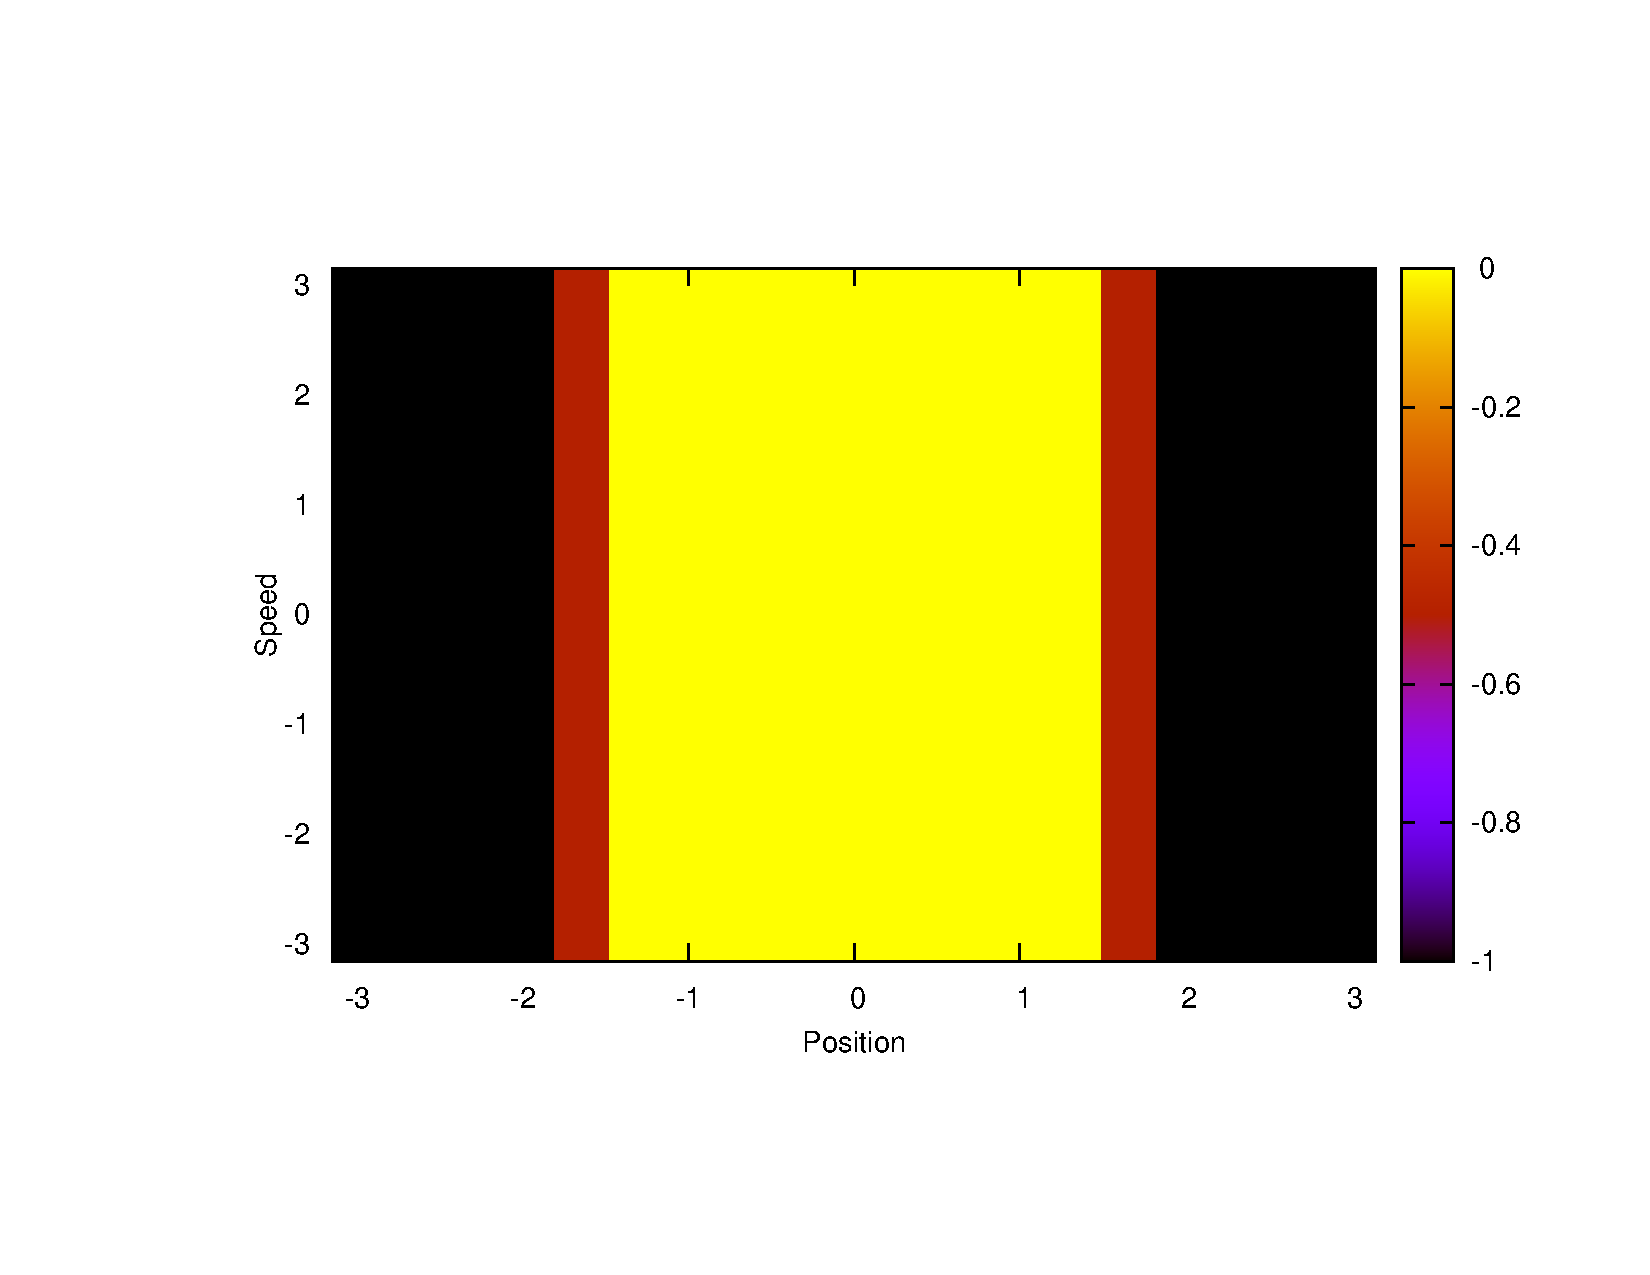
\includegraphics[width=1.2\linewidth]{LAFEM_Exp3_true_R.pdf}}
  \centerline{(a) Récompense de l'expert}%\medskip
\end{minipage}
\hfill
\begin{minipage}[b]{.5\linewidth}
  \centering
  \centerline{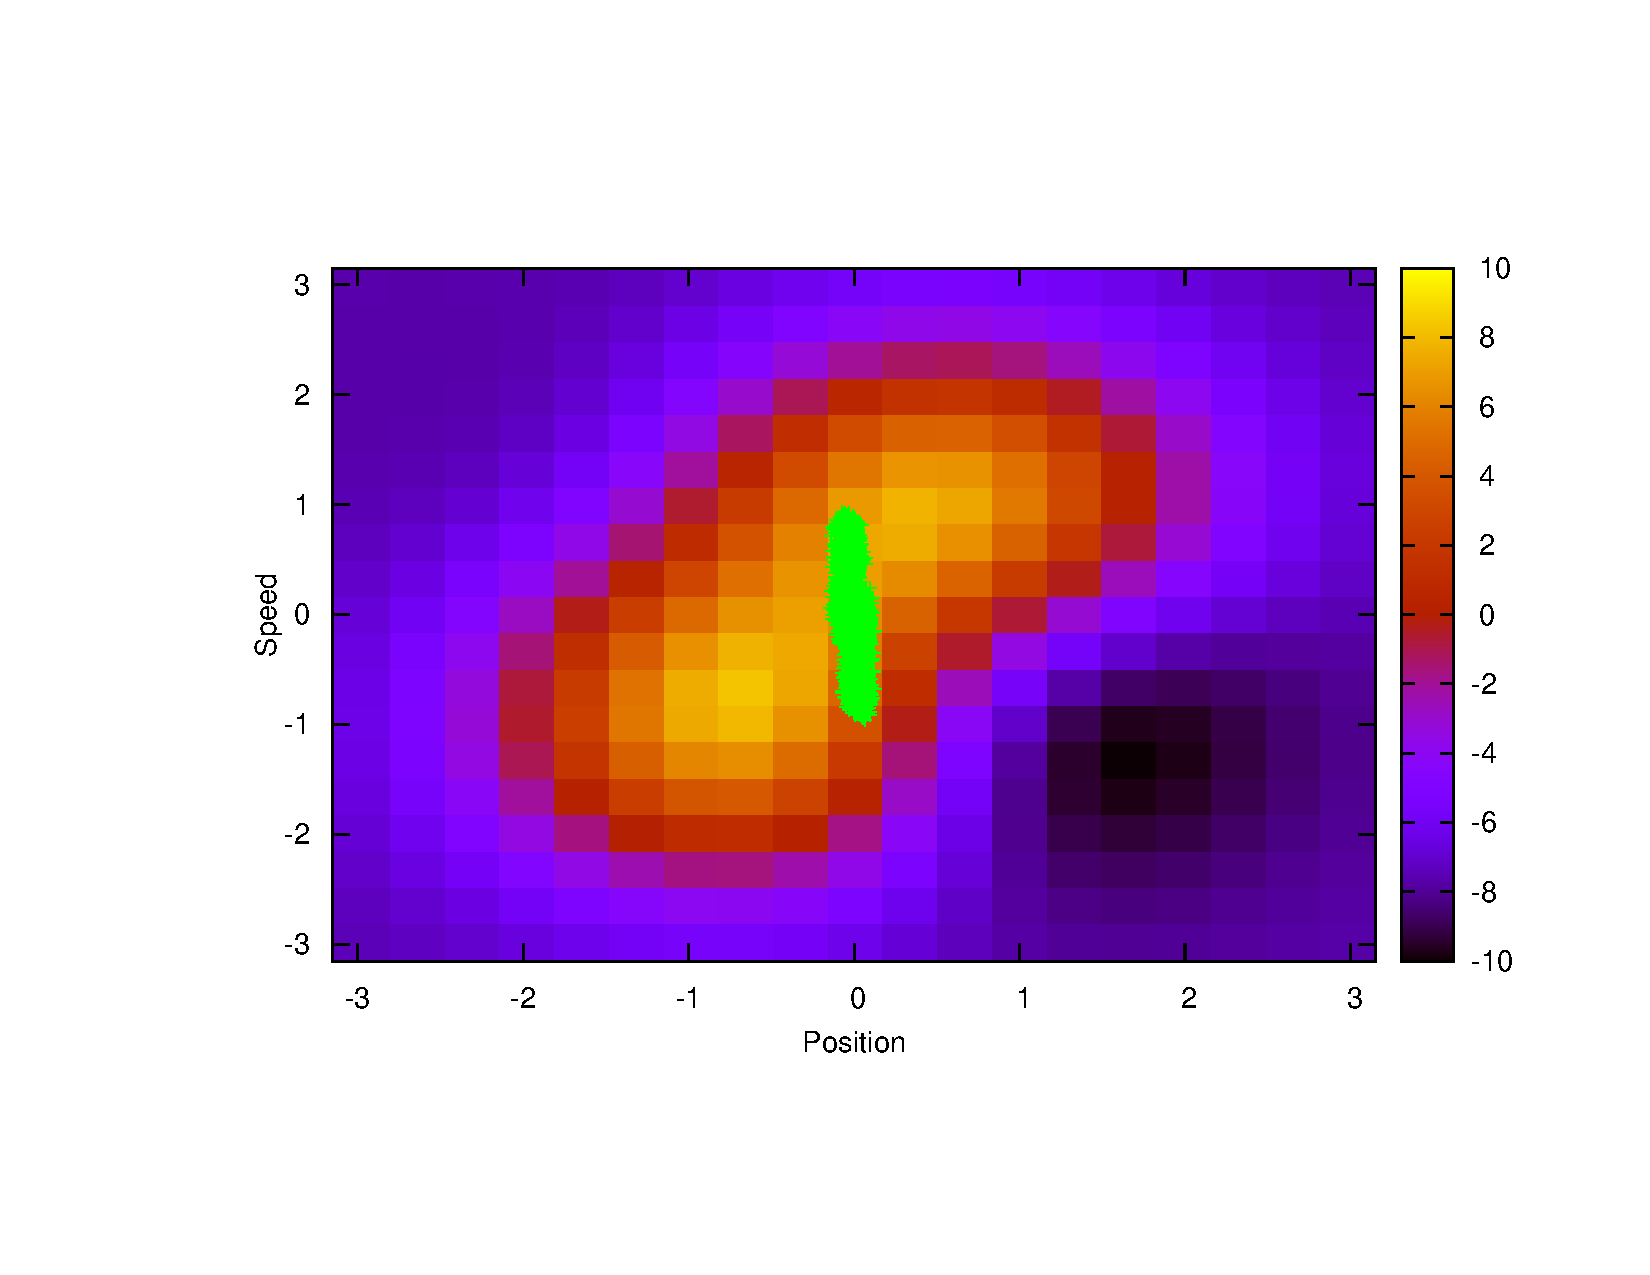
\includegraphics[width=1.2\linewidth]{LAFEM_Exp3_lafem_R.pdf}}
  \centerline{(b) Récompense trouvée}%\medskip
\end{minipage}
\begin{minipage}[b]{.5\linewidth}
  \centering
  \centerline{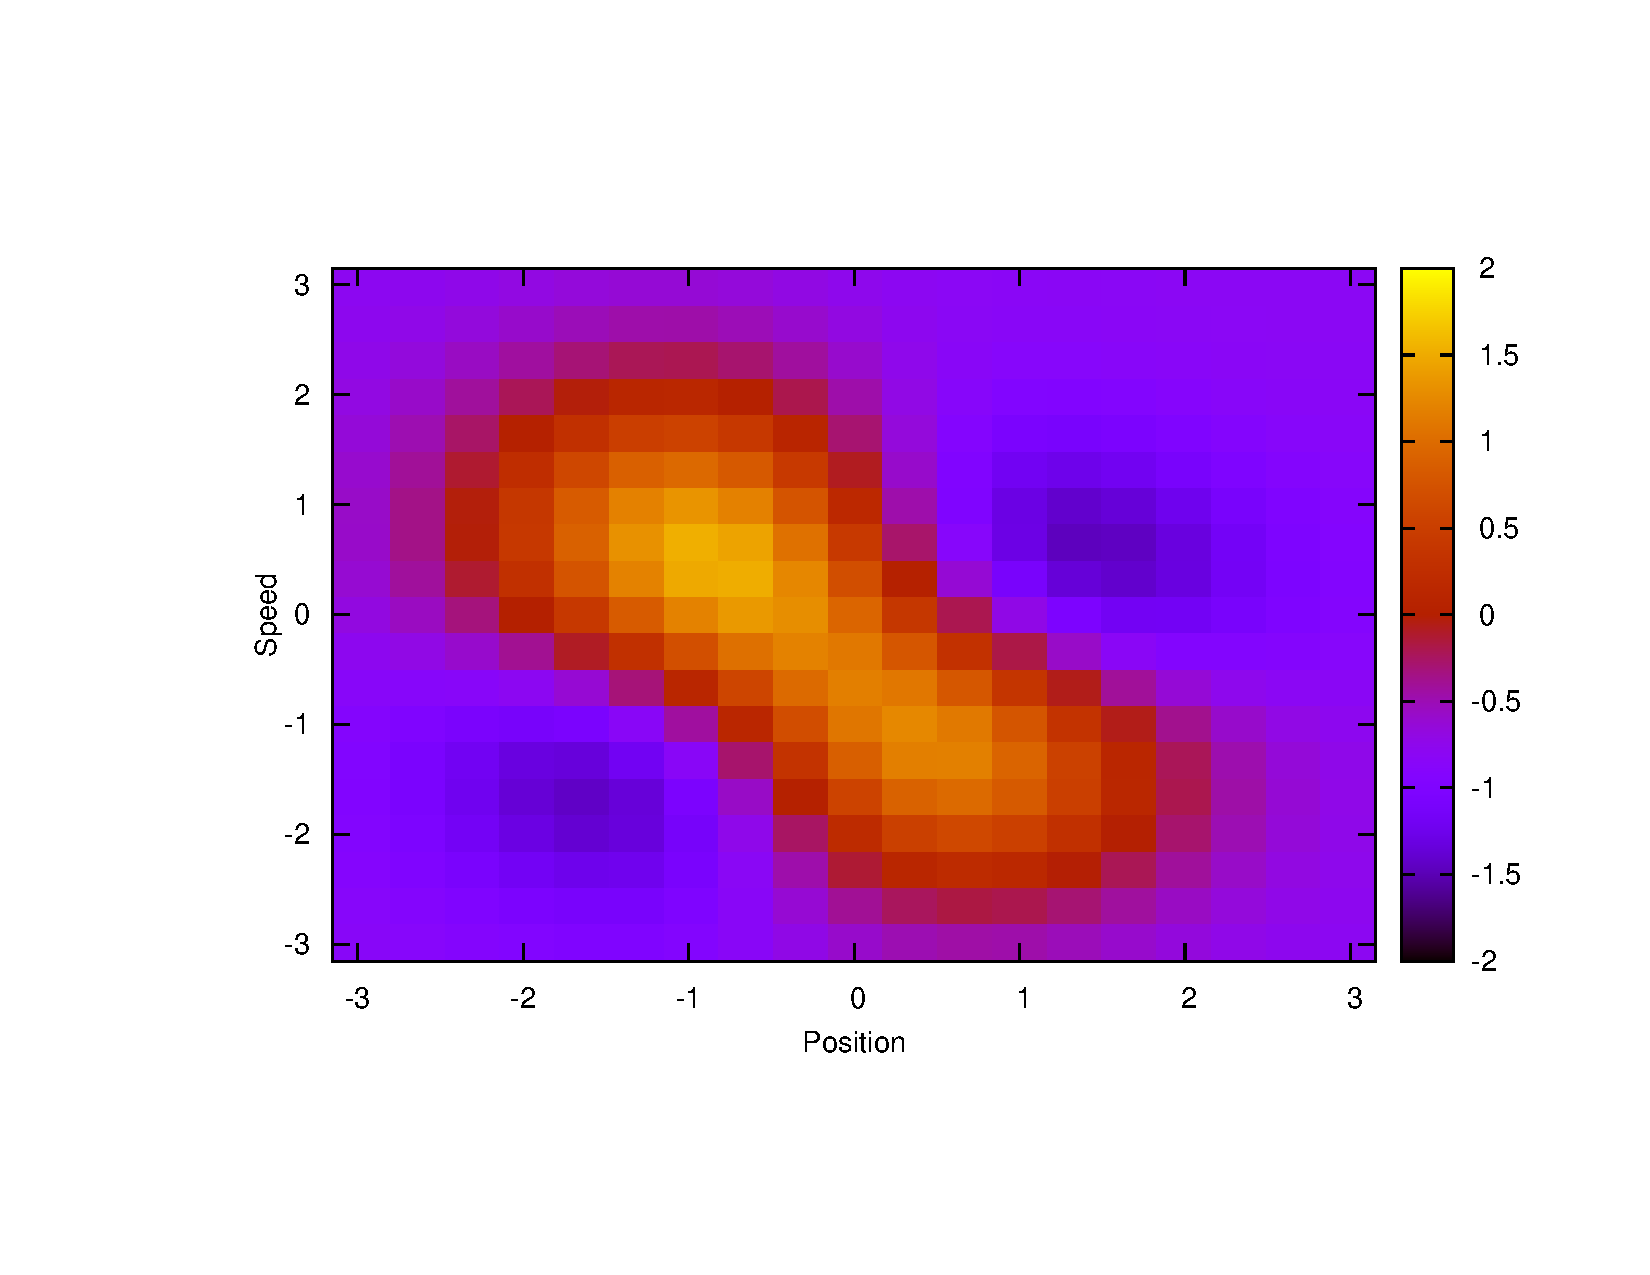
\includegraphics[width=1.2\linewidth]{LAFEM_Exp3_Vexpert.pdf}}
  \centerline{(c) Fonction de valeur de l'expert}%\medskip
\end{minipage}
\hfill
\begin{minipage}[b]{.5\linewidth}
  \centering
  \centerline{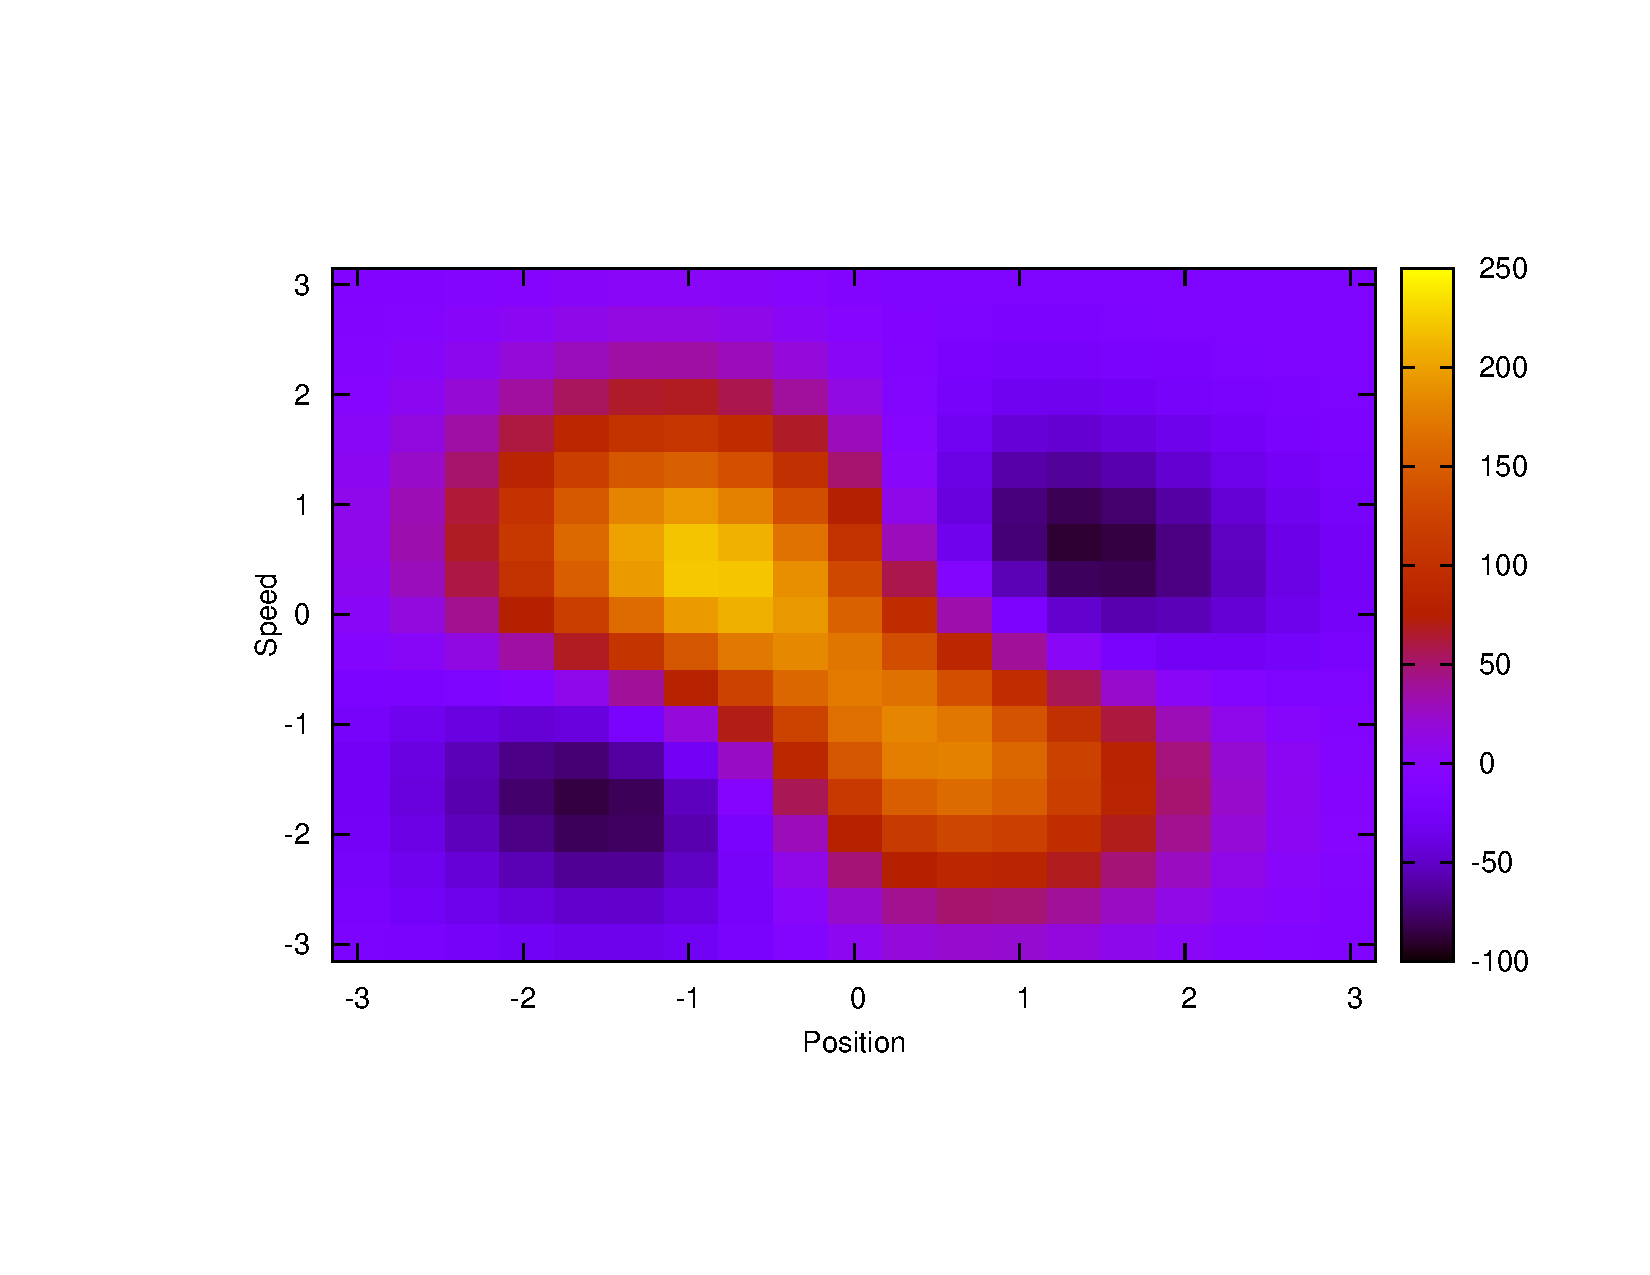
\includegraphics[width=1.2\linewidth]{LAFEM_Exp3_Vagent.pdf}}
  \centerline{(d) Fonction de valeur de l'agent}%\medskip
\end{minipage}
%
\caption{Résultats fournis par notre algorithme.}
\label{onlyFig.fig}
%
\vspace{-5pt}
\end{figure}

Afin d'étudier le comportement de notre algorithme, nous avons fait générer à l'expert une base de données $D_E$ de transitions contenant 10 trajectoires de 300 transitions chacune. La fonction $l$ fut définie sur les états présents dans $D_E$ telle que $l(s,a) = 0$ si $a=\pi_E(s)$, $1$ sinon. Le pas de temps est constant à $\alpha_t = 0.1$ et le nombre d'itérations est de $T=20$. Le vecteur initial $\theta_0$ fut fixé à $[-1...-1]^T$, la récompense étant paramétrée à l'aide du vecteur d'attribut $\psi : S \rightarrow \mathbb{R}^p$ correspondant au mélange de gaussiennes défini dans \cite{lagoudakis2003least}. Pour l'approximation de l'attribut vectoriel moyen de l'expert, c'est l'algorithme LSTD$\mu$ qui fut employé.\\


Si la fonction de récompense trouvée par LAFEM (figure \ref{onlyFig.fig} (b)) diffère de celle fournie à l'expert (figure \ref{onlyFig.fig} (a)) on constate en revanche que les fonctions de valeurs sont très similaires (figures \ref{onlyFig.fig} (c) et \ref{onlyFig.fig} (d)). Cela est une illustration du fait que le problème de l'ARI est mal posé en ceci qu'il n'y a pas qu'une seule récompense pouvant expliquer une politique.\\

Avec le nombre d'échantillons fournis par l'expert (3000 en 10 trajectoires de 300 transitions chacune), l'agent parvient systématiquement à maintenir le pendule en équilibre durant 5 minutes, ce qui est notre critère de réussite.\\

Deux éléments méritent d'être notés. Tout d'abord la faible couverture de l'espace d'état offerte par les échantillons de l'expert. Ceux-ci sont portés en vert sur la Figure \ref{onlyFig.fig} (b) et l'on constate qu'ils n'occupent qu'une toute petite partie de l'espace : celle dans laquelle le pendule est proche de la verticale. En l'absence de données dans le reste de l'espace d'état il n'est pas possible de pouvoir y inférer avec certitude la récompense. Le second point à noter est que la "vraie" récompense ne se trouve pas dans l'espace d'hypothèse que notre algorithme explore, en effet les attributs vectoriels utilisés ne peuvent qu'approximer la fonction de récompense utilisée sans l'atteindre. Malgré ces deux difficultés, notre algorithme parvient, comme nous l'avons dit, à extraire une récompense qui permet à un agent d'obtenir des performances similaires à celles de l'expert. Le lecteur attentif aura noté la différence d'amplitude des fonctions de valeur Fig. \ref{onlyFig.fig} Cela n'a aucune importance, une dilatation laissant la politique optimale invariante.
\section{Conclusion}

L'algorithme présenté dans cette contribution lève les problèmes les plus contraignants de l'apprentissage par renforcement inverse. En rendant la résolution du problème inverse indépendante de celle du problème direct, nous sommes en mesure d'inférer une récompense cohérente avec le comportement d'un expert en mode purement \emph{batch}.\\

Comme nous l'avons illustré, les échantillons nécessaires à la réussite de notre algorithmes sont faciles à recueillir. Une simple trace de l'expert, même si elle ne couvre qu'une petite partie de l'espace d'état, suffit à inférer une récompense. Cette récompense, description compacte de la tâche effectuée par l'expert, peut alors être optimisée par un agent dont les capacités diffèrent de celles de l'expert. On rentre dans le cadre du \emph{transfer learning}.\\

L'estimation de $mu_E$ est centrale dans notre approche. Nous disposons d'un algorithme efficace avec LSTD$\mu$, mais qui présente cependant les mêmes inconvénients que les algorithmes d'estimation d'une fonction de valeur. L'axe d'étude que nous envisageons d'explorer serait de ne plus passer par l'attribut vectoriel moyen en trouvant le moyen d'introduire autrment la structure du PDM dans la démarche de classification que nous avons adoptée. Des tests empiriques sur des problèmes plus comlpexes sont également envisagés.
%
% Bibliographie
%
\bibliography{Biblio}

\end{document}

